\documentclass[../thesis.tex]{subfiles}

\begin{document}

\intro \label{chapter:intro}

\renewcommand{\epigraphrule}{0pt}
\setlength{\afterepigraphskip}{6pt}
\epigraph{Fully secure systems don't exist today and they won't exist in the future.}{\textit{Adi Shamir}}

В последнее время наблюдаются высокие темпы роста применения облачных технологий и виртуальных инфраструктур.
Новые технологии изменили и усложнили природу компьютерных сетей --- облака и крупные центры обработки данных (ЦОД) предъявляют к сетям повышенные требования.
Операторам требуются более «умные» сети, а также усовершенствования в инструментах сетевого мониторинга и управления.

Программно-конфигурируемые сети\footnote{Software-Defined Networking (SDN) – англ.} (ПКС), по мнению ведущих производителей сетевого оборудования, являются одним из самых перспективных направлений сетевой индустрии на данный момент \cite{kreutz2015software}.
ПКС – это концепция построения сети, в которой контур управления сетью (\textit{control-plane}) отделен от контура передачи данных (\textit{data-plane}).
Согласно концепции ПКС, вся логика управления переносится на отдельное устройство --- контроллер, который способен отслеживать работу всей сети и управлять сетевыми устройствами --- коммутаторами.

Наиболее важный аспект концепции ПКС --- логически централизованное управление сетью, которое обеспечивает глобальное видение топологии и состояния управляемой сети как на уровне L2, так и на уровне L3.
Контроллер собирает информацию о характеристиках коммутаторов, топологии сети, загрузке физических линий и об установленных соединениях между хостами (пользовательскими устройствами).
В отличие от традиционных сетей, в которых каждое устройство имеет собственное представление о состоянии сети, в ПКС сети контроллер имеет полную информацию о состоянии сети, и, таким образом, предоставляет централизованную платформу для реализации логики управления сетью.

В среде контроллера, подобно традиционным операционным системам, работают приложения, которые используют сервисы контроллера для управления различными ресурсами сети.
Такие приложения могут выполнять множество функций, например, управлять маршрутизацией пакетов, контролировать доступ к сетевым ресурсам, балансировать нагрузку в сети и т.п.
Контролер предоставляет приложениям унифицированный, открытый интерфейс и сервисы по управлению программируемой сетевой инфраструктурой.
Благодаря контроллеру, сеть, состоящая из множества коммутаторов разных производителей, предстает для приложения как один логический коммутатор.
Такой подход дает более удобные абстракции для разработчиков сетевых приложений по сравнению с сетями с традиционной архитектурой.

Одним из важных элементов концепции ПКС является протокол\linebreak OpenFlow \cite{mckeown2008openflow, openflow15} для программирования и управления коммутаторами.
Схема работы протокола представлена на рисунке \ref{fig:openflow}.

\begin{figure}
\centering
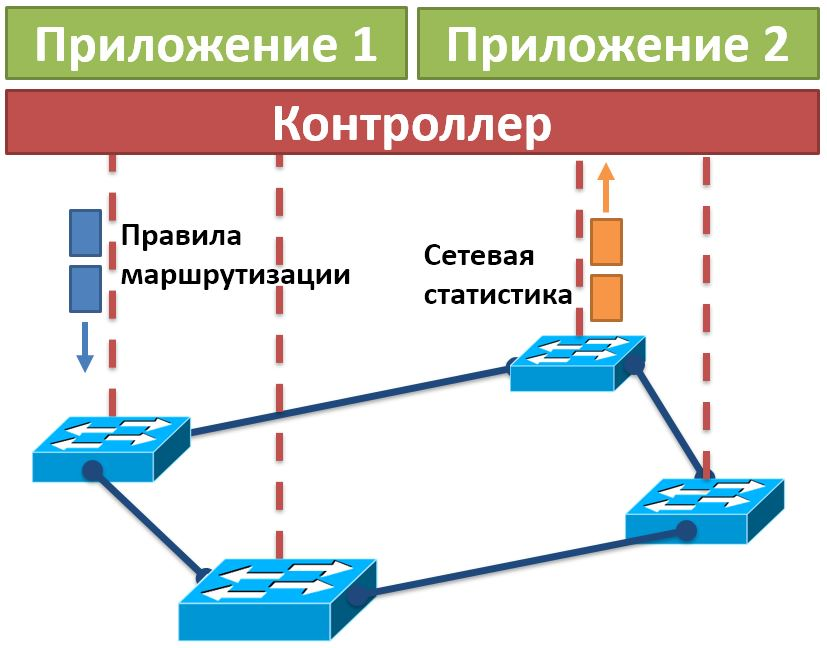
\includegraphics[width=0.6\textwidth]{figures/openflow.jpg}
\caption{Схема работы протокола OpenFlow} \label{fig:openflow}
\end{figure}

Протокол OpenFlow предполагает использование на коммутаторах специальных таблиц маршрутизации, в которые контроллер загружает правила для маршрутизации (рис. \ref{fig:flowtable}) и/или модификации пакетов, проходящих через коммутатор.
Такие таблицы называются таблицами потоков (\textit{flow}-таблицами).
Каждый коммутатор имеет несколько таблиц потоков, которые образуют конвейер обработки пакета.
Конвейер обработки пакета используется для последовательной обработки пакетов несколькими правилами маршрутизации.
Каждая таблица потоков имеет уникальный номер, начиная с нуля.

Протокол OpenFlow также позволяет загружать правила в специальную выделенную таблицу маршрутизации, называемую групповой таблицей.
Записи в групповой таблице называются групповыми правилами маршрутизации.
Групповые правила маршрутизации дублируют (зеркалирующее) трафик и производят различные действия с каждой копией пакета в отдельности.
Действия над копиями пакета описываются записями, называемыми \textit{bucket}-записями.
Протокол OpenFlow также описывает опциональные групповые правила маршрутизации, которые не обязательно должны быть реализованы на коммутаторах.
Эти опциональные групповые правила не дублируют пакеты на каждую \textit{bucket}-запись, вместо этого они выбирают \textit{bucket}-запись по специальному алгоритму выбора.

Пакеты, поступившие на входной буфер коммутатора, сначала проверяются на соответствие их заголовков шаблонам правил из нулевой таблицы.
Заголовки пакетов сравниваются с шаблонами правил в порядке убывания приоритета правила, и если заголовок совпадает с шаблоном, то выполняется инструкция, связанная с выбранным правилом.
Такими инструкциями могут быть: отправка пакета на некоторый порт, сброс пакета или отправка пакета на контроллер для дальнейшего анализа.
Также пакеты могут быть отправлены в таблицу потоков с большим номером, где они будут обработаны другим правилом маршрутизации.

Записями каждой таблицы потоков являются правила маршрутизации, представленные в виде кортежа \textit{<match, priority, counter, action>} (рис. \ref{fig:flowrule}).
Каждая bucket-запись представляет собой правило маршрутизации без полей \textit{<match>} и \textit{<priority>}.

\begin{figure}
\centering
\begin{subfigure}[b]{0.4\textwidth}
  \centering
  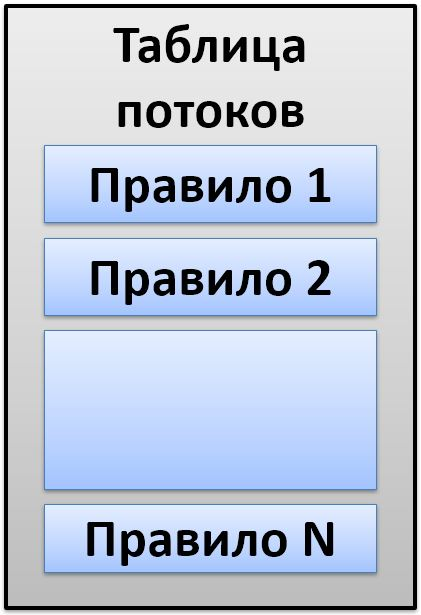
\includegraphics[width=0.8\textwidth]{figures/flowtable.jpg}
  \caption{Таблица потоков} \label{fig:flowtable}
\end{subfigure}
\begin{subfigure}[b]{0.4\textwidth}
  \centering
  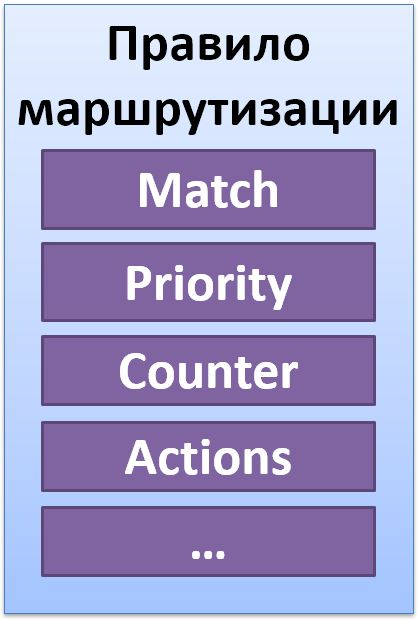
\includegraphics[width=0.8\textwidth]{figures/flowrule.jpg}
  \caption{Правило маршрутизации} \label{fig:flowrule}
\end{subfigure}
\caption{Примитивы протокола OpenFlow}
\end{figure}

\begin{itemize}
\item Поле \textit{<match>} описывает множество пакетов, которые могут обрабатываться этим правилом.
\item Поле \textit{<priority>} используется для разрешения неопределенностей обработки пакетов, то есть, если в таблице есть несколько правил, шаблонам которых соответствует пакет, то выбирается правило с наивысшим приоритетом.
Спецификация протокола OpenFlow прямо указывает, что наличие правил с одинаковым приоритетом и пересекающимися полями \textit{<match>} ведет к неопределенному поведению.
\item Поле \textit{<counter>} описывает количество пакетов, обработанных правилом маршрутизации с момента его установки на коммутатор.
\item Поле \textit{<action>} описывает набор действий с пакетами.
Действиями могут быть: сброс пакета, отправка на контроллер, отправка в таблицу потоков или групповую таблицу, отправка на порт и изменение заголовка пакета.
\end{itemize}

Сети, построенные по концепции ПКС, обладают рядом свойств, которые хорошо подходят для построения безопасной и управляемой вычислительной среды:
\begin{itemize}
\item Разделение контура управления (\textit{control}-plane) и контура передачи данных (\textit{data}-plane) позволяет изолировать логику управления сетевыми устройствами.
\item Парадигма потока данных более удобна для обеспечения безопасности, поскольку она предлагает сквозную (\textit{end-to-end}) модель связей, ориентированную на сервисы, не связанную с традиционными ограничениями маршрутизации.
\item Логически централизованное управление позволяет во всей сети осуществлять эффективную защиту и мониторинг появления угроз.
\item Переход к программному управлению позволяет осуществлять динамичную и гибкую настройку политики безопасности.
\end{itemize}

В случае построения сети по концепции ПКС ряд угроз безопасности становятся не актуальными, часть механизмов защиты может быть реализована в коммутаторах и контроллере \cite{chao2016securing}.
Например, концепция ПКС предоставляет гибкие возможности по сегментированию и изоляции узлов сети \cite{kreutz2015software}.
Некоторые атаки, использующие слабости протоколов маршрутизации, могут быть исключены, так как в ПКС многие протоколы не используются, однако в случае гибридной сети они могут контролироваться средствами ПКС \cite{scott2013sdn}.

Несмотря на это, с появлением новой концепции компьютерных сетей появляются и новые виды угроз, которые могут привести не только к материальным потерям, но и к утрате репутации и имиджа компаний, использующих подобные сети \cite{kloti2013openflow}.
Следовательно, во избежание негативных последствий компьютерных атак, необходимо производить анализ защищенности ПКС и разрабатывать механизмы защиты таких сетей.
\\

Угрозы для сетей, построенных по концепции ПКС, можно описать следующим образом:

1) \textit{Угрозы безопасности канала данных}

Этот тип угроз аналогичен угрозам безопасности канала данных в традиционных сетях.
Он заключается в том, что если у злоумышленника есть доступ к каналу данных, то он может производить атаку \textit{Man-in-the-Middle} на пользовательский трафик \cite{desmedt2011man}.

Разделяют два вида атаки \textit{Man-in-the-Middle}: пассивная и активная.
При пассивной атаке злоумышленник перехватывает пользовательский трафик и анализирует его на предмет наличия важных данных, таких как персональная информация, пароли и т.п.

Активная атака предполагает изменение пользовательского трафика.
Например, злоумышленник может вставлять вредоносный код в Web-страницы, возвращаемые сервером пользователю.
\\
\\

2) \textit{Угрозы безопасности коммутаторов}

Как и в любом программном или аппаратном обеспечении, в ПКС коммутаторах могут присутствовать уязвимости \cite{chao2016securing, garcia2014analysis}.
Эти уязвимости могут быть проэксплуатированы злоумышленником для получения контроля над коммутатором \cite{thimmaraju2016reins}.

Более того, концепция ПКС предполагает возможность использования программных коммутаторов.
Такие коммутаторы могут быть установлены на серверы общего назначения, на которых одновременно с коммутатором работают другие приложения, имеющие уязвимости.
И как следствие, эксплуатация уязвимости в одном из таких приложений может привести к компрометации всего сервера, и в том числе ПКС коммутатора.

Компрометация коммутатора является серьезной проблемой, которая создает угрозу компрометации всей сети, так как атакующий может использовать подконтрольные ему коммутаторы для проведения широкого спектра атак как на пользовательский трафик, так и на сетевые устройства \cite{neti2012software}.
\\

3) \textit{Угрозы безопасности канала управления}

Этот тип угроз является специфичным для концепции ПКС, так как в ней канал управления отделен от канала передачи данных.
Если у злоумышленника есть доступ к каналу управления, то он может перехватывать и изменять управляющий трафик, посылаемый как контроллером коммутатору, так и наоборот.
Таким образом, злоумышленник может нарушать взаимодействие контроллера с коммутаторами в сети, изменяя перехваченные пакеты.

Успешность таких атак на контур управления напрямую зависит\linebreak от используемой защиты управляющего трафика.
Спецификация протокола OpenFlow \cite{openflow15} предполагает защиту управляющего трафика при помощи протокола TLS \cite{turner2014transport}.
Такая защита необходима для того, чтобы злоумышленник не мог перехватывать и изменять управляющий трафик.
Несмотря на то, что использование протокола TLS описано в спецификации протокола OpenFlow, этот пункт не является обязательным.
Это приводит к возможности появления в сети ошибок администрирования, когда защита не была включена администратором, и злоумышленник может получить доступ к управляющему трафику.

Угроза безопасности управляющего трафика также может возникнуть из-за уязвимостей как в протоколе TLS \cite{sheffer2015summarizing, meyer2013lessons}, так и в его реализации \cite{durumeric2014matter}.
\\

4) \textit{Угрозы безопасности контроллера}

Компрометация контроллера влечет за собой компрометацию всей сети, которой он управляет \cite{scott2013sdn}.
Обычных методов обнаружения вторжения здесь может быть недостаточно, так как зачастую весьма сложно установить комбинацию событий, вызывающих конкретное поведение, при такой атаке, и, кроме того, доказать, что оно вредоносное \cite{wang2018towards}.
\\

5) \textit{Угрозы безопасности приложений}

Для того, чтобы реализовывать логику управления сетью, приложения на контроллере получают доступ к разного рода операциям, в том числе и критическим.
Как и любое программное обеспечение, приложения могут содержать ошибки, которые могут привести к незапланированному поведению приложения, например, к его аварийному завершению.
Более того, использование сторонних приложений может привести к угрозе запуска вредоносной программы с правами управления сетью \cite{shin2014rosemary}.
\\

В настоящей работе рассматривается задача обнаружения скомпрометированных ПКС коммутаторов.
Под скомпрометированным ПКС коммутатором понимается коммутатор сети, управляемой ПКС контроллером, который, в действительности, находится под контролем злоумышленника.
Возможность компрометации коммутаторов обусловлена тем, что коммутаторы могут иметь уязвимости \cite{garcia2014analysis, myerson2002identifying, skaggs2002network}, которые могут быть проэксплуатированы злоумышленником для получения над ними контроля.

Одним из примеров уязвимости в ПКС коммутаторе, которая может\linebreak привести к его компрометации некоторым злоумышленником, является\linebreak \textit{CVE-2016-2074} \cite{thimmaraju2016reins} в коммутаторах \textit{Open vSwitch} \cite{pfaff2015design} версии ниже, чем 2.4.1.
Эта уязвимость заключается в том, что злоумышленник может создать специальный пакет с большим количеством MPLS \cite{davie2000mpls} меток и отправить этот пакет на коммутатор.
Обработка такого пакета приведет к переполнению буфера и выполнению произвольного кода на коммутаторе.

Несмотря на то, что все функции управления сетью вынесены на контроллер, компрометация коммутатора является серьезной угрозой безопасности всей сети, так как атакующий может использовать подконтрольные ему коммутаторы для проведения различных атак как на контур данных, так и на контур управления \cite{neti2012software}.

Одним из основных методов проведения атаки на \textit{data-plane} при помощи скомпрометированного ПКС коммутатора является установка злоумышленником дополнительных правил маршрутизации \cite{pang2016fade}.
Поскольку концепция ПКС дает большую свободу в управлении сетевым трафиком, злоумышленник может реализовать произвольную логику атаки на сеть: сбрасывать трафик из заранее выбранных потоков, дублировать трафик на некоторый хост для дальнейшего анализа или изменять заголовки пакета так, чтобы они были сброшены на другом легитимном коммутаторе.

Злоумышленник также может проводить атаки на \textit{control-plane}.
К таким атакам относятся атаки, влияющие на информацию о сети, хранимую на контроллере \cite{hong2015poisoning}.
Так как всю информацию о сети контроллер получает от коммутаторов, злоумышленник может отправлять на контроллер некорректные данные о состоянии сети.
Например, атакующий может отправить контроллеру информацию о несуществующей в сети физической линии.
Это может привести к тому, что некоторые потоки будут направлены по такой несуществующей линии и в итоге будут сброшены коммутатором, что приведет к отказу в обслуживании.
\\

Сложность задачи обнаружения скомпрометированного коммутатора заключается в том, что подобный коммутатор невозможно обнаружить средствами аутентификации устройства.
Это обусловлено тем, что, получая контроль над коммутатором, злоумышленник получает доступ к криптографическим ключам, находящимся в памяти коммутатора.
Далее, используя эти ключи, злоумышленник сможет провести процедуру аутентификации скомпрометированного коммутатора.
А любой коммутатор, прошедший процедуру аутентификации, будет считаться легитимным с точки зрения контроллера \cite{openflow15}.
Таким образом, необходимы методы проверки различных признаков компрометации коммутаторов.

Одним их основных признаков компрометации ПКС коммутатора является наличие на коммутаторе правил маршрутизации, которые не были установлены контроллером \cite{dhawan2015sphinx} (рис. \ref{fig:comprimizedswitch}).
Так как ПКС коммутатор не может сам устанавливать правила маршрутизации, то наличие подобных правил говорит о том, что их установил злоумышленник.

\begin{figure}
\centering
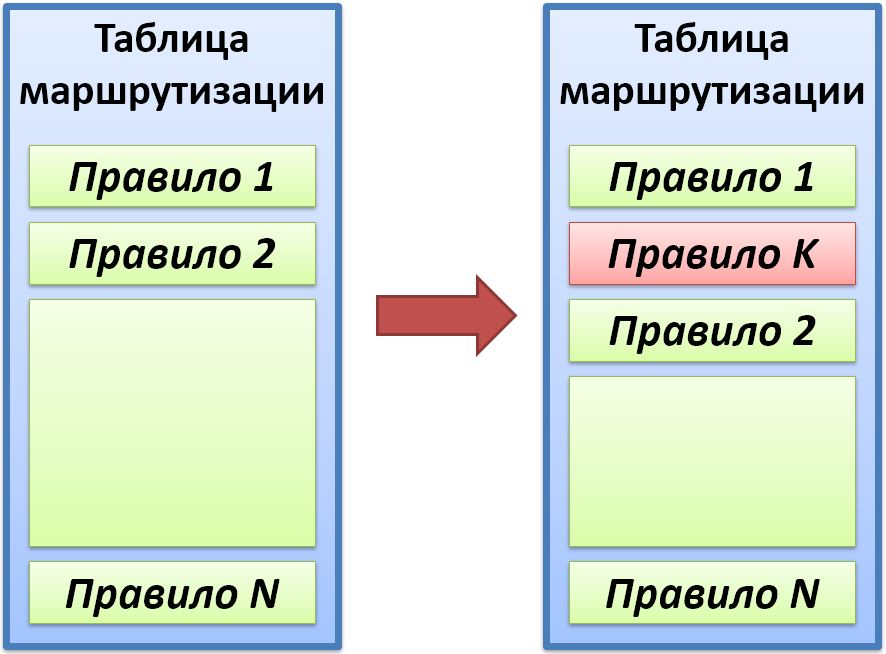
\includegraphics[width=0.6\textwidth]{figures/comprimizedswitch.jpg}
\caption{Скомпрометированный коммутатор} \label{fig:comprimizedswitch}
\end{figure}

Для проверки наличия несанкционированных правил на коммутаторе, контроллер должен хранить копию правил, которые он установил на каждый коммутатор.
Далее контроллер может считывать с коммутаторов информацию о всех правилах маршрутизации, которые установлены в таблицах маршрутизации.
Таким образом, контроллер имеет информацию о том, какие правила должны быть на каждом коммутаторе, и может сравнивать их с реальными правилами, находящимися в памяти коммутатора.

Слабостью такого подхода является то, что злоумышленник может подделывать информацию о правилах маршрутизации, отправляемую на контроллер.
Например, он может создать две таблицы с правилами маршрутизации: в одну будут сохраняться все правила, устанавливаемые легитимным контроллером, а в другую, правила, устанавливаемые злоумышленником.
Назовем такие таблицы \textit{основной} и \textit{теневой}.

Наличие двух таблиц может быть использовано злоумышленником для обхода описанного выше механизма защиты.
Если контроллер запросит хранящиеся на коммутаторе правила, то коммутатор предоставит ему правила из \textit{основной} таблицы, но для обработки реального сетевого трафика будут использоваться правила из \textit{теневой} таблицы.

Следовательно, контроллер не сможет проверить наличие на коммутаторе лишних правил, потому что коммутатор будет предоставлять контроллеру некорректные данные о реально используемых для обработки трафика правилах.

На основании вышесказанного следует, что необходимы методы, которые позволят обнаружить скомпрометированные коммутаторы по различным косвенным признакам, то есть по наличию атак на контур передачи данных и по влиянию этих атак на легитимные коммутаторы.
   
\pagebreak

\section*{Цель диссертационной работы}
\addcontentsline{toc}{section}{Цель диссертационной работы}
    
Целью диссертационной работы является разработка алгоритма обнаружения скомпрометированных коммутаторов в ПКС.

Для достижения поставленной цели в рамках настоящей работы было необходимо решить следующие задачи:

\begin{enumerate}
\item Провести обзор и сравнительный анализ существующих средств обнаружения скомпрометированных ПКС коммутаторов.
\item Разработать математическую модель ПКС сети для описания динамики изменения счетчиков правил маршрутизации.
\item Разработать алгоритм предсказания значения счетчиков правил маршрутизации, основанный на разработанной математической модели, и доказать его корректность.
\item Разработать алгоритм обнаружения скомпрометированных ПКС коммутаторов, который будет использовать алгоритм предсказания значений счетчиков правил маршрутизации, и обосновать его корректность.
\end{enumerate}

\section*{Актуальность работы}
\addcontentsline{toc}{section}{Актуальность работы}

Актуальность работы определяется растущей популярностью концепции ПКС в качестве сетевой архитектуры как для сетей центров обработки данных (ЦОД) \cite{kreutz2015software}, так и для сетей телеком-операторов (\textit{Metro-WAN}) \cite{jain2013b4}, наличием угрозы компрометации коммутаторов в таких сетях \cite{chao2016securing, garcia2014analysis}, а также отсутствием систем обнаружения скомпрометированных коммутаторов в ПКС, которые бы не накладывали ограничений на логику работы приложений на контроллере.

\section*{Научная новизна}
\addcontentsline{toc}{section}{Научная новизна}

В диссертации разработана новая математическая модель, описывающая динамику изменения счетчиков правил маршрутизации в ПКС, в рамках которой сделана математическая постановка задачи.
На основе математической модели был разработан новый алгоритм предсказания значений счетчиков правил маршрутизации при произвольной логике работы приложений на контроллере.
Также был проведен анализ известных алгоритмов обнаружения скомпрометированных коммутаторов в ПКС, на основании которого сформулированы основные ограничения существующих алгоритмов.

В диссертации предложен новый алгоритм обнаружения скомпрометированных коммутаторов в ПКС, который свободен от ограничений существующих алгоритмов.

\section*{Теоретическая и практическая значимость}
\addcontentsline{toc}{section}{Теоретическая и практическая значимость}
Теоретическая значимость работы состоит в проведении обзора существующих систем обнаружения скомпрометированных коммутаторов в ПКС, построении математической модели, описывающей изменение счетчиков правил маршрутизации, разработке алгоритма предсказания значений счетчиков правил маршрутизации и алгоритма обнаружения скомпрометированных коммутаторов в ПКС.

Практическая значимость работы обусловлена тем, что результаты работы могут быть использованы для обеспечения безопасности в сетях телеком-операторов и центрах обработки данных.

\section*{Положения, выносимые на защиту}
\addcontentsline{toc}{section}{Положения, выносимые на защиту}

\begin{itemize}
\item Впервые разработана математическая модель, описывающая динамику изменения счетчиков правил маршрутизации в OpenFlow коммутаторах в ПКС, которая инвариантна к набору правил маршрутизации, установленных в OpenFlow коммутаторах, и логике работы приложений контроллера в ПКС.

\item В рамках разработанной модели построен алгоритм предсказания значений счетчиков правил маршрутизации, корректность которого доказана.

\item На основе алгоритма предсказания значений счетчиков построен алгоритм обнаружения скомпрометированных коммутаторов, для которого экспериментально получены оценки ошибок первого/второго рода и время обнаружения скомпрометированных коммутаторов на топологиях, используемых в сетях операторов связи и центров обработки данных.
Показано, что представленный алгоритм обнаружения превосходит известные алгоритмы обнаружения, используемые в существующих системах обнаружения, по ряду практически важных критериев.
\end{itemize}

\section*{Апробация работы}
\addcontentsline{toc}{section}{Апробация работы}

Результаты, представленные в работе, докладывались на научных семинарах лаборатории Вычислительных комплексов кафедры Автоматизации систем вычислительных комплексов факультета ВМК МГУ под руководством чл.-корр. РАН, профессора Р.Л. Смелянского, семинаре кафедры Автоматизации систем вычислительных комплексов имени чл.-корр. РАН, профессора Л.Н. Королёва, научном семинаре кафедры Математической кибернетики факультета ВМК МГУ под руководством доктора физ.-мат. наук, профессора В.А. Захарова, заседании консорциума «ПКС в научно образовательной среде», проводимом Центром Прикладных Исследований Компьютерных Сетей, а также на 5 конференциях:
\begin{enumerate}
\item Всероссийской научной конференции «Ломоносовские чтения --- 2017»
\item Международной научной конференции «REDS-2017»
\item Международной научной конференции «ElConRus-2018»
\item Всероссийской научной конференции «Ломоносовские чтения --- 2018»
\item Международной научной конференции «MoNeTec-2018»
\end{enumerate}

\section*{Публикации}
\addcontentsline{toc}{section}{Публикации}

Основные результаты по теме диссертации изложены в 1 патенте на изобретение \cite{petrov2018patent} и в 12 печатных изданиях \cite{petrov2017problem, petrov2017detection, petrov2017control, petrov2017maninthemiddle, petrov2018detection, petrov2018minimizationrus, petrov2018minimization, petrov2018mathematical, petrov2018forwarding, petrov2018anonymity, petrov2019survey, petrov2019forwardingrus}.
5 публикаций \cite{petrov2018minimization, petrov2018mathematical, petrov2018forwarding, petrov2019survey, petrov2019forwardingrus} изданы в журналах, рекомендованных ВАК, 3 из них \cite{petrov2018minimization, petrov2018mathematical, petrov2018forwarding} изданы в журналах, цитируемых Scopus / Web of Science.

В работе \cite{petrov2017control} вклад Шемякина Р.О. заключается в реализации системы обеспечения контроля доступа приложений к ресурсам контроллера и проведении экспериментального исследования.
Петрову И.С. принадлежит постановка задачи и описание алгоритма обеспечения контроля доступа.

В работе \cite{petrov2017maninthemiddle} Шендяпин А.С. реализовал тестовые атаки Man-in-the-Middle с использованием скомпрометированного коммутатора и провел экспериментальное исследование.
Вклад Петрова И.С. заключается в постановке задачи, разработке методов проведения тестовых атак и описании методики проведения экспериментального исследования.

В работах \cite{petrov2018detection, petrov2018minimizationrus, petrov2018minimization} вклад Смелянского Р.Л. заключается в постановке задач и описании методик проведения экспериментов.
Петрову И.С. принадлежит разработка алгоритмов минимизации группового трафика и обнаружения скомпрометированных коммутаторов, обзоре существующих решений, реализации алгоритмов и проведении экспериментальных исследований.

В работе \cite{petrov2018forwarding} Моргунова О.М. реализовала алгоритм минимизации количества правил маршрутизации и провела экспериментальное исследование.
Вклад Петрова И.С. заключается в разработке алгоритма минимизации количества правил маршрутизации для анализа сетевой статистики и описании методики проведения экспериментального исследования.

В работе \cite{petrov2018anonymity} Шендяпину А.С. принадлежит экспериментальное сравнение существующих средств обеспечения анонимности в программно-конфигурируемых сетях.
Петрову И.С. принадлежит описание критериев сравнения и проведение обзора существующих средств.

В патенте \cite{petrov2018patent} вклад Смелянского Р.Л. и Шалимова А.В. заключается в постановке задачи и описании методики анализа алгоритма минимизации группового трафика.
Петрову И.С. принадлежит проведение обзора существующих решений и разработка алгоритма минимизации группового трафика в программно-конфигурируемых сетях.

\section*{Личный вклад автора}
\addcontentsline{toc}{section}{Личный вклад автора}

Все представленные в диссертации результаты получены лично автором.

\section*{Структура работы}
\addcontentsline{toc}{section}{Структура работы}

{
\hypersetup{linkcolor=black}
Диссертация состоит из введения, 6 глав, заключения и 1 приложения.

\hyperref[chapter:intro]{\textbf{Во введении}} обоснована актуальность диссертационной работы, сформулирована цель и аргументирована научная новизна исследований, показана практическая значимость полученных результатов, представлены выносимые на защиту научные положения и дано краткое описание задачи.

\hyperref[chapter:problem]{\textbf{В первой главе}} приводится постановка задачи обнаружения скомпрометированных коммутаторов в ПКС.

\hyperref[chapter:classification]{\textbf{Во второй главе}} приведено описание атак, которые злоумышленник может производить при помощи скомпрометированного ПКС коммутатора.

\hyperref[chapter:survey]{\textbf{В третьей главе}} проводится обзор существующих систем обнаружения скомпрометированных коммутаторов в ПКС, выделяются их основные недостатки и также определяются требования к разработке системы обнаружения скомпрометированных коммутаторов.

\hyperref[chapter:model]{\textbf{В четвертой главе}} проводится описание разработанной математической модели ПКС сети, описывающей динамику изменения счетчиков правил маршрутизации в сети с произвольной комбинацией установленных правил маршрутизации.

\hyperref[chapter:algorithm]{\textbf{В пятой главе}} приведено описание разработанного алгоритма обнаружения скомпрометированых коммутаторов в ПКС.

\hyperref[chapter:implementation]{\textbf{В шестой главе}} представлено описание разработанного прототипа системы обнаружения скомпрометированных коммутаторов и результаты его экспериментального исследования.

\hyperref[chapter:conclusion]{\textbf{В заключении}} формулируются основные результаты работы.

\hyperref[chapter:appendix]{\textbf{В приложении А}} подробно описаны компоненты разработанной системы обнаружения скомпрометированных коммутаторов.
\\

Полный объём диссертации составляет \ref{TotPages} страниц с \total{figurenum} рисунками и\linebreak \total{tablenum} таблицами.
Список литературы содержит \total{citenum} наименования.
}

\end{document}